% Main document: main.tex. Compiler: pdfLaTeX.
% COMP3019J Web Application Development — Milestone 1: Design
\documentclass[11pt,a4paper]{article}
\usepackage[margin=22mm]{geometry}
\usepackage[T1]{fontenc}
\usepackage[utf8]{inputenc}
\usepackage{lmodern,microtype,enumitem,titlesec,graphicx,caption,array,tabularx}
\newcolumntype{Y}{>{\raggedright\arraybackslash}X}
\renewcommand{\arraystretch}{1.2}
\usepackage[hidelinks]{hyperref}
\captionsetup{hypcap=false}
\setlength{\parindent}{0pt}
\setlength{\parskip}{6pt}
\renewcommand{\baselinestretch}{1.08}
\setlist[itemize]{leftmargin=1.4em,itemsep=2pt,topsep=3pt,parsep=0pt}
\setlist[enumerate]{leftmargin=1.6em,itemsep=4pt,topsep=3pt,parsep=0pt}
\titleformat{\section}{\large\bfseries}{\thesection}{0.65em}{}
\titlespacing*{\section}{0pt}{12pt}{6pt}
\pagestyle{plain}
\clubpenalty=10000
\widowpenalty=10000
\raggedbottom
\newcommand{\prompt}[1]{\textit{#1}}
\newcommand{\reportheader}[3]{%
\begin{center}
{\small\bfseries COMP3019J Web Application Development}\par
\vspace{2pt}\hrule\vspace{9pt}
{\LARGE\bfseries #1}\par
\vspace{2pt}Design Report
\end{center}
{\small\textbf{Team:} #2\par
\textbf{Members:} #3\par}
\vspace{3pt}}

\begin{document}

\reportheader{Food Delivery Website}{xLLM}
{Fu Rao (24107744), Liu Jing (24107741), Liu Zongrun (24107745), Zhou Jiaxu (24107758)}

\section{Project Idea}

A local food delivery service connects three parties: customers who order meals, several
independent restaurants that cook them, and delivery riders who collect and deliver them. The
difficulty is not that any one of these actions is hard. It is that the service has to operate
while its own facts keep changing, and that the three parties never see the same thing.

Each restaurant controls its own opening times, menu and preparation capacity, and all three
change during the day: a dish sells out, the kitchen becomes busy, a shop closes early. An order
is only fulfilled if the restaurant and the rider coordinate two separate physical steps ---
preparing the food and collecting it --- and the customer stands outside both of them with no
way of knowing what is happening. In practice this produces three recurring failures. The
participants duplicate work or wait on each other; the customer telephones the restaurant to ask
where the order is, which the restaurant cannot answer either; and the normal path breaks
whenever there is a delay, an unavailable dish, a wrong address or a cancellation. There is also
a privacy problem underneath: giving all three parties the same view would show one customer
another customer's home address, show one restaurant another restaurant's orders, and expose
rider contact details to everyone.

The service we will build therefore has to do two things at once: hold the order as a
\emph{shared record} that all three parties work on, and give each party a different view of
that record according to what they are responsible for.

\noindent\textbf{User roles.} We identify three roles. Their needs differ, and so do their
permissions --- the difference is the core of the design, not an afterthought.

\begin{itemize}
\item \textbf{Customer.} Needs to order food from a nearby restaurant and to know when it will
arrive. May create orders, read and cancel \emph{their own} orders and write a review. Must
never see another customer's orders or address, a restaurant's internal workload, or a rider's
personal details.
\item \textbf{Restaurant staff.} Need to receive orders, prepare them, and hand them over.
May manage \emph{their own} opening hours, menu items and availability, and move \emph{their
own} orders through preparation. Must never see another restaurant's orders or menu, and may
not alter the amounts charged on an order.
\item \textbf{Delivery rider.} Needs to find work and complete deliveries. May see the pool of
orders that are prepared and unclaimed, claim one, report position, and move that order through
delivery. Must never see orders that are not ready, or orders another rider has claimed.
\end{itemize}

\noindent\textbf{Why it is useful.} The application covers the whole life of an order, not a single step, and replaces telephone
coordination with one shared record each party can act on, so the exception paths are explicit.

\section{Main Functions}

The first five functions are \emph{essential}: without them the central workflow cannot be
demonstrated. The rest are \emph{optional}
additions, attempted once the essential set works end to end.

\begin{itemize}
\item \textbf{F1 --- Accounts and roles.} Each role registers and signs in through its own
interface; all three share one authentication module and one session, and the role decides what that
session may reach. Result: an authenticated session that the server uses to
authorise every later request.
\item \textbf{F2 --- Restaurant menu and hours.} Restaurant staff set opening hours per weekday,
add and edit dishes with price, calories and remaining stock, and mark a dish unavailable.
Result: the public menu always reflects what the kitchen can actually produce now.
\item \textbf{F3 --- Browsing and ordering.} A customer browses restaurants, selects a delivery
address by pointing at a map, and places an order containing several dishes. Result: an order
record holding a \emph{snapshot} of the address and of each dish's name and price.
\item \textbf{F4 --- Order progression.} Restaurant staff accept an order, mark it preparing and
then ready; a rider claims the ready order, confirms collection and confirms delivery. Result:
the order advances through defined states, and the same record is updated by two different
roles in turn.
\item \textbf{F5 --- Order tracking.} The customer sees their own orders and the current state
and timestamps of each. Result: progress is visible without contacting the restaurant.
\item \textbf{F6 --- Reviews (optional).} After delivery the customer rates the restaurant and
the rider from one to five stars with a comment. Result: a quality signal attached to a
completed order.
\item \textbf{F7 --- Rider location (optional).} A rider reports position while delivering and
the customer sees it on a map. Result: live progress rather than a status label.
\item \textbf{F8 --- Coupons (optional).} A customer claims and applies a discount at checkout.
Result: a discounted total recorded on the order.
\end{itemize}

\noindent\textbf{Priority.} F1--F5 are the minimum for a coherent demonstration: only these
take one order from request to delivery through two roles. F6--F8 add value but the topic does
not require them, so they come last and are cut first.

\noindent\textbf{Rules that constrain these functions.}
\begin{itemize}
\item \emph{Ownership.} A record may only be changed by the party that owns it: a dish by its
own restaurant, an order by its own customer, restaurant or rider. The check is made on the
server for every query, not by hiding controls in the interface.
\item \emph{Transition authority.} Apart from cancellation, each state change belongs to exactly one
role: only the restaurant may accept and prepare, and only a rider may collect and deliver. No role may skip a
state.
\item \emph{Claim exclusivity.} An order enters the rider pool only when it is ready and has no
rider. Claiming is a single conditional update, so if two riders act at the same moment exactly
one succeeds and the other is told the order has gone.
\item \emph{Cancellation window.} The customer may cancel while the order is placed or accepted,
because nothing has been cooked yet. Once the kitchen starts preparing, only the restaurant may
cancel, and it records why.
\item \emph{Delivery range.} An order is refused if the selected address lies outside the
restaurant's configured delivery radius, and the customer is told why.
\item \emph{Record integrity.} Address and prices are copied into the order when it is placed.
Later edits to an address or a menu therefore cannot rewrite the history of past orders.
\end{itemize}

\section{Application Design}

\noindent\textbf{Application structure.} Figure~\ref{fig:structure} shows the main parts.
Three browser interfaces --- customer, restaurant and rider --- send requests over HTTPS to a
reverse proxy, which forwards every request --- pages as well as \texttt{/api} --- to the
application server. The
application is divided into functional modules, one per business domain. The
\emph{authentication module} establishes the caller and their role.
The \emph{restaurant module} manages shop profiles, opening hours and menu items. The
\emph{order module} creates orders and enforces the state machine, and is the only module that
writes order states. The \emph{rider module} manages the claimable pool and position reports.
The \emph{review module} records ratings against completed orders. All modules share one data
access layer, so ownership checks are written in one place. The database holds the records in Table~\ref{tab:data}. Two external
services are used: a map service, loaded by the browser to pick addresses and to draw a rider's
position; and a mail service, used only for one-time codes (code sign-in and password reset). The
delivery radius is checked by the server itself, without the map service.

\begin{figure}[h]
\centering
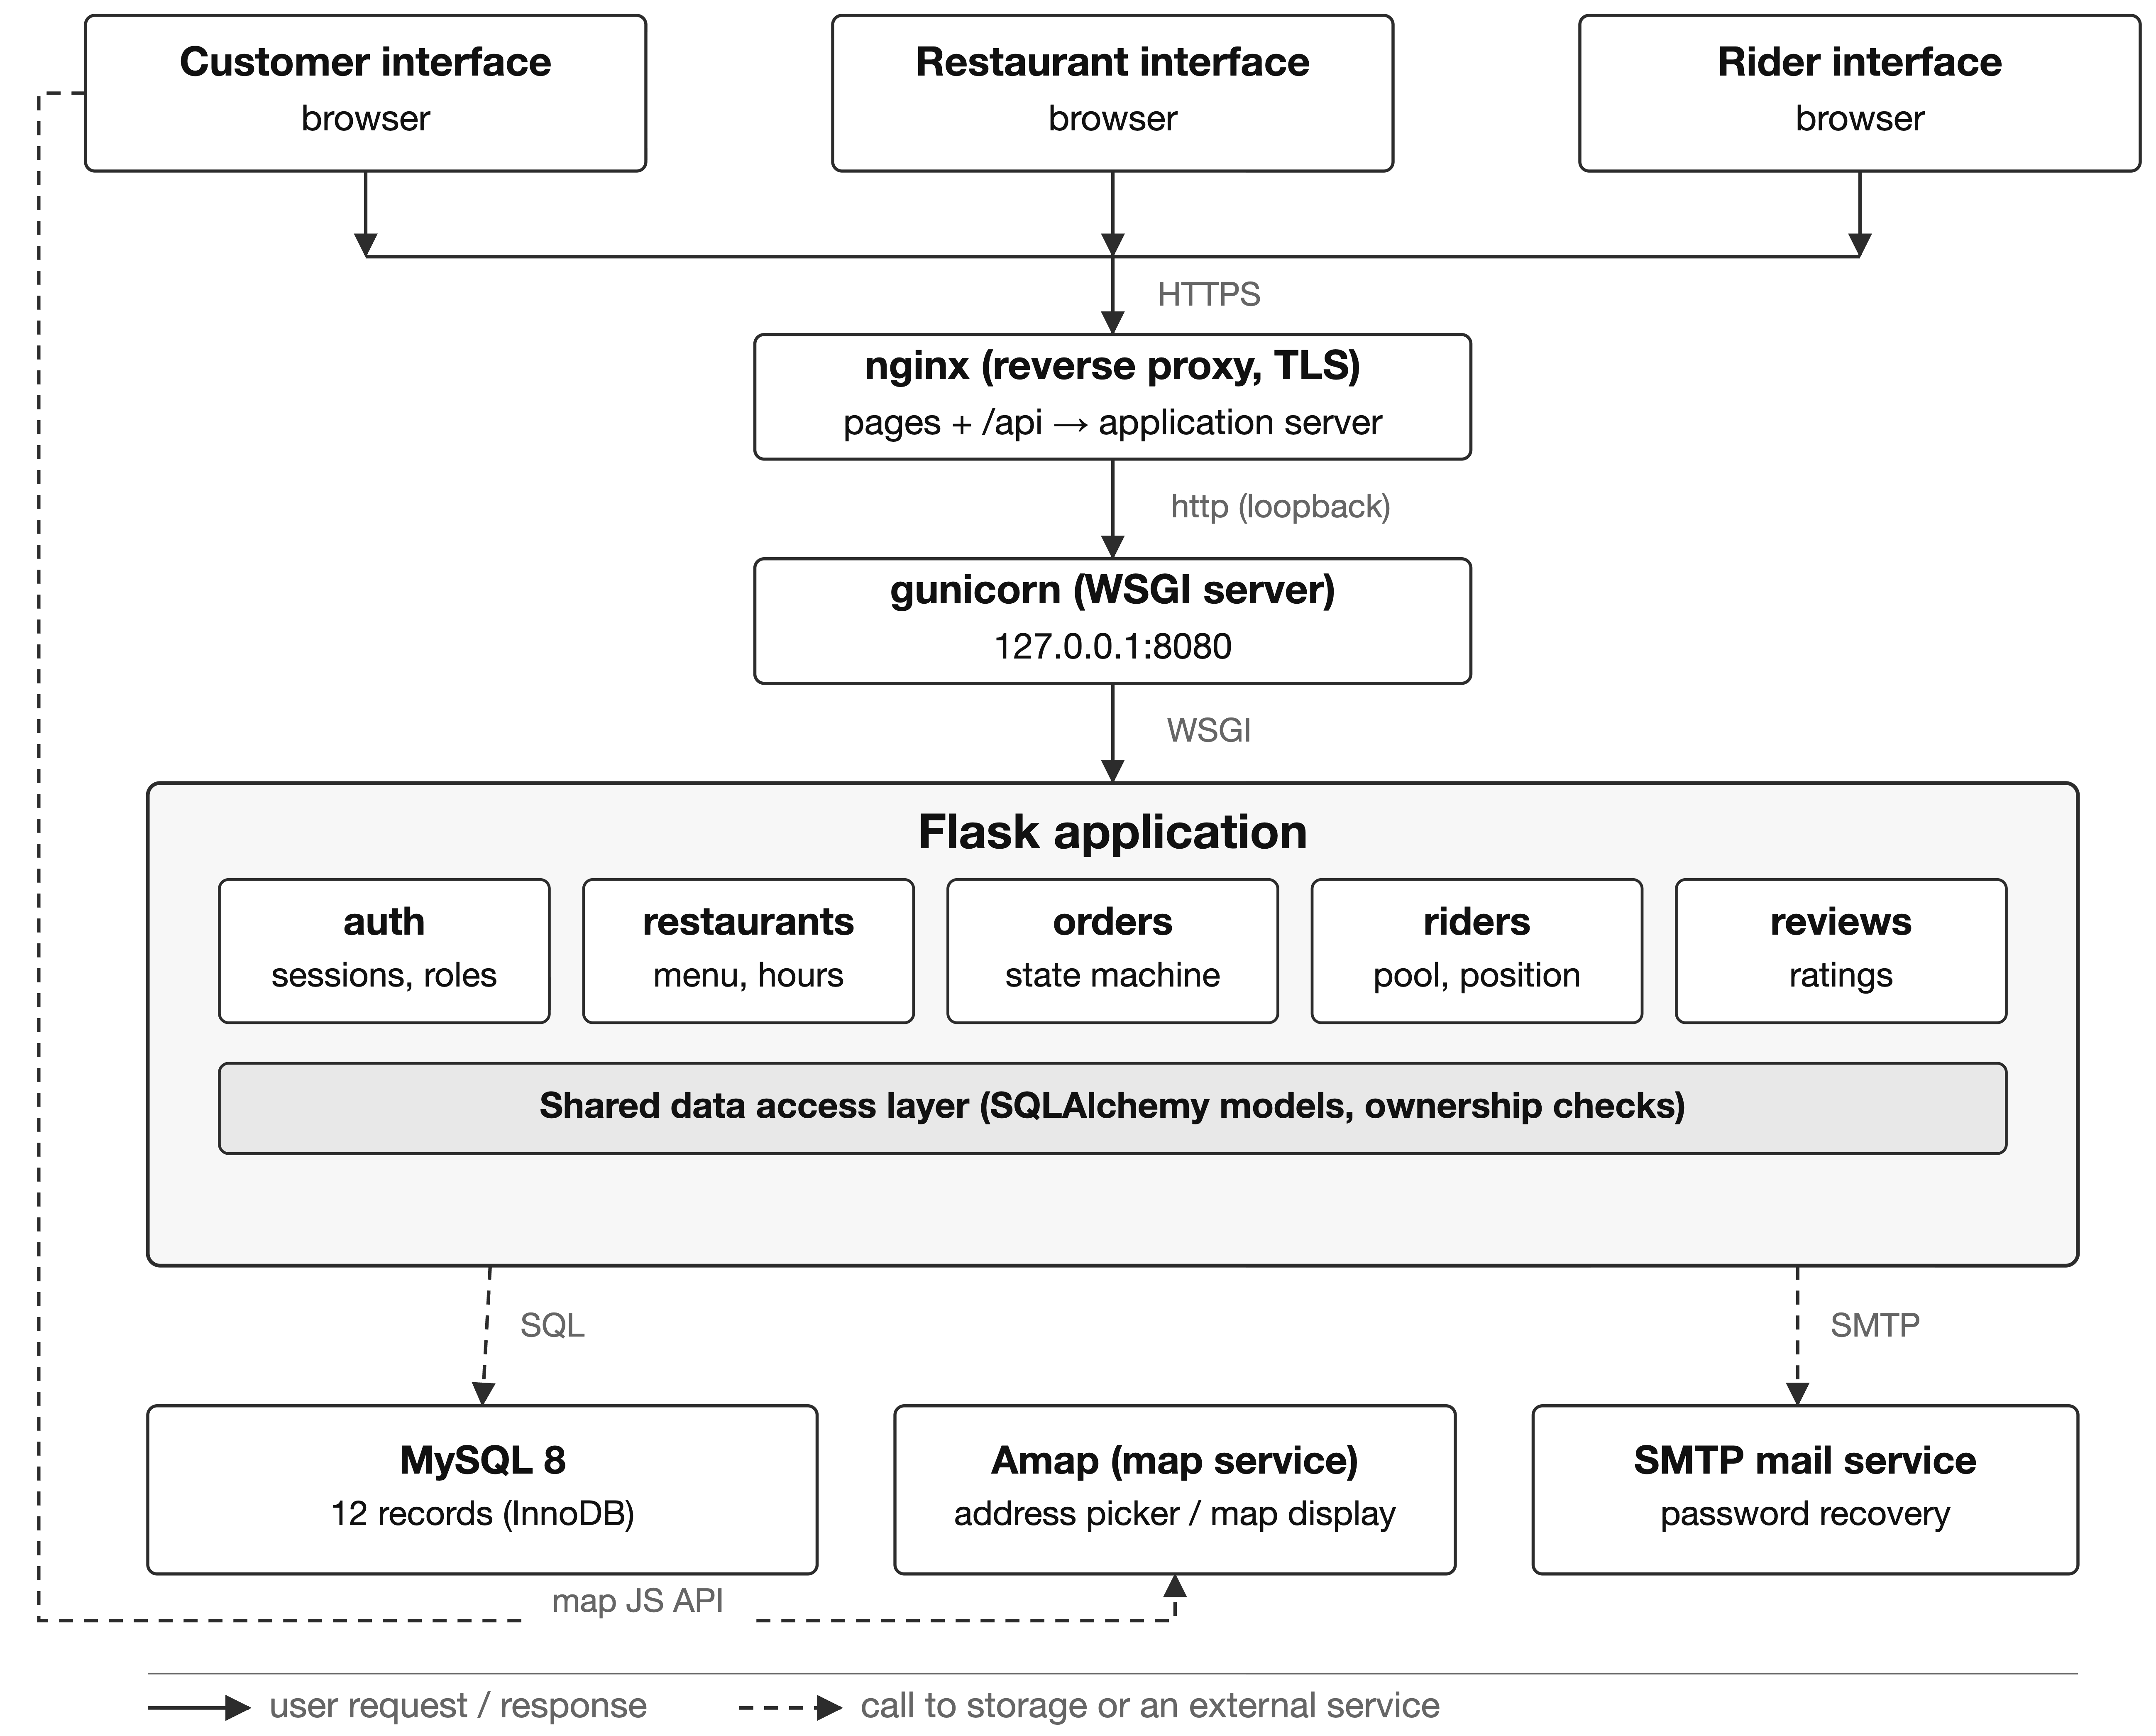
\includegraphics[width=0.66\linewidth]{structure.png}
\caption{Main parts of the application. Solid arrows carry user requests and responses over
HTTPS; the dashed arrows show calls to the database, to the mail service, and --- from the
browser --- to the map service.}
\label{fig:structure}
\end{figure}

\noindent\textbf{Data.} Table~\ref{tab:data} lists the records the application stores, the
information in each, and the functions that use or update them.

\begin{table}[h]
\footnotesize
\renewcommand{\arraystretch}{1.0}
\begin{tabularx}{\linewidth}{|p{27mm}|Y|Y|}
\hline
\textbf{Record}&\textbf{Information stored}&\textbf{Functions that use or update it}\\\hline
Users & Role, username, e-mail, display name, hashed password &
F1 creates and authenticates; every other function reads it to decide permissions.\\\hline
Restaurants & Owner, name, address and coordinates, delivery radius, minimum order, open flag &
F2 updates it; F3 reads it to list shops and check the delivery radius.\\\hline
Rider profiles & Rider, online flag, vehicle type, service radius &
F1 creates it; F4 refuses a claim unless the rider is online.\\\hline
Opening hours & Restaurant, weekday, open and close time, closed flag &
F2 maintains; F3 uses it to refuse orders outside opening hours.\\\hline
Menu items & Restaurant, name, price, calories, stock, available flag &
F2 maintains; F3 reads for display and copies price into the order.\\\hline
Addresses & Customer, label, contact, address text, coordinates, default flag &
F1 owns them; F3 selects one and copies it into the order.\\\hline
Orders & Customer, restaurant, rider, state, address and amount snapshots, distance, timestamps &
F3 creates; F4 and F5 update and read the state; F6 attaches a review to it.\\\hline
Order items & Order, dish reference, name and price snapshots, quantity &
F3 writes them; F4 reads them to show the kitchen what to cook.\\\hline
Reviews & Order, reviewer, target, rating, comment &
F6 creates; F2 and F5 read ratings back.\\\hline
Rider locations & Rider, order, coordinates, accuracy, timestamp &
F7 appends them; F5 reads the latest one for display.\\\hline
Coupons and claims & Code, owner, discount, threshold, claim status &
F8 issues, claims and redeems them against an order.\\\hline
Verification codes & E-mail, purpose, hashed code, expiry, attempts &
F1 sends and checks them for code sign-in and password resets.\\\hline
\end{tabularx}
\caption{Records, the information stored in each, and the functions that use them.}
\label{tab:data}
\end{table}

\noindent\textbf{How the records connect.} An \emph{order} is the record that links the parties:
it names the customer who placed it, the restaurant that must cook it and --- once claimed ---
the rider who delivers it, so all three roles act on the same row. An order owns many
\emph{order items}, one per dish; each item points at a \emph{menu item} but also carries its own
copy of the name and price, which is what allows the menu to change without altering history. A
\emph{restaurant} owns its hours and its menu items, and a \emph{customer} owns a list of
addresses; the chosen address is copied into the order for the same reason. A \emph{review} is
attached to a delivered order and names its target --- the restaurant or the rider --- and the
order alone is what proves the reviewer was entitled to write it. \emph{Rider locations} are
appended against an order while it is being delivered.

\noindent\textbf{User workflow.} Consider the task of placing and fulfilling one order.

\begin{enumerate}
\item The customer signs in (F1). The authentication module reads \emph{users}, starts a
session and returns the role, which selects the customer interface.
\item The customer opens a restaurant (F3). The restaurant module reads \emph{restaurants},
\emph{opening hours} and \emph{menu items} and returns only those items currently available.
\item The customer picks a delivery address on the map and adds dishes to a cart. The map
service converts the chosen point into coordinates and a readable address.
\item The customer confirms. The order module checks the distance against the restaurant's
radius, then writes one \emph{orders} row with the address and total copied in, plus one
\emph{order items} row per dish with name and price copied in. The order starts in state
\emph{pending}. Result: the customer can now see progress (F5), and the restaurant can see the
order (F4).
\item The restaurant accepts, marks it preparing, then ready. Each step updates the
\emph{orders} row and stamps the matching timestamp; only the restaurant that owns the order may
do this.
\item The order now appears in the rider pool. A rider claims it --- a single conditional update
that succeeds only if the order is still ready and still unclaimed --- then confirms collection
and later delivery. The \emph{orders} row moves to \emph{delivering} and then \emph{delivered}.
\item The customer sees the final state and may leave a review (F6), which is written against
this order.
\end{enumerate}

\emph{A situation that changes the process: cancellation.} Suppose the customer wants to cancel
\emph{after} the kitchen has started preparing the food. The normal path offers no free way out,
because ingredients have already been committed. The order module therefore refuses the
customer's cancellation and tells them to contact the restaurant, whose decision it is. If the
restaurant agrees, the order moves to \emph{cancelled}, with the cancelling party and reason
recorded alongside the timestamp; it disappears from the restaurant's queue and from the rider
pool, and any payment is marked refunded. If the restaurant refuses, the order simply continues
along the normal path. The same rule covers the reverse timing: while the order is still
\emph{pending} or \emph{accepted} nothing has been cooked, so the customer cancels directly. The rule is thus a property of the order's state, not of the
interface the request arrived from.

\section{Technology Choices}

\noindent\textbf{Browser.} HTML5 and CSS3 for structure and presentation; JavaScript with the
browser's \texttt{fetch} API for interaction and for calling the server without reloading the
page; Jinja2 templates
on the server to render the three role interfaces. The browser presents and validates input,
including the map that captures coordinates.

\noindent\textbf{Server.} Python 3.10 with Flask 3.1, using Werkzeug password hashing and Flask
sessions, with SQLAlchemy 2.0 as the data access layer. The server is where the application
actually lives: it authenticates every request, decides per record whether the caller is
entitled to read or change it, runs the order state machine, and is the only part that holds
database credentials.

\noindent\textbf{Data storage.} MySQL 8 with InnoDB and \texttt{utf8mb4}, holding the twelve
records in Table~\ref{tab:data}. A relational store is the right fit because the rules above are
relational: ownership is a column on the row, claim exclusivity is \emph{one} conditional
\texttt{UPDATE} guarded by \texttt{rider\_id IS NULL}, duplicate ratings for the same order
and target are refused, and per-order history is preserved by copying values rather than joining to live
ones. Foreign keys keep the order graph consistent while a record is passed between roles.

\noindent\textbf{Why this combination suits the project.} One language for the server and the
data layer keeps the ownership checks in one place; server-rendered pages with asynchronous requests keep the three interfaces simple while still allowing
progress to refresh without a reload; and the relational model expresses the topic's own
language --- availability, ownership, approval --- directly as constraints.

\noindent\textbf{Technology not covered in class.}

\begin{itemize}
\item \emph{Map service (Amap)} --- used to let a customer point at a delivery address instead
of typing it, and to check the delivery radius. The benefit is direct: hand-typed addresses are
the main source of the address problems the topic names, and pointing at a map removes that
ambiguity at source. Management: one browser key, restricted by domain and paired with a security
code, is the only credential exposed; the radius check uses straight-line distance computed
locally, so no server-side key is needed, the ordering flow still works if the service is
unavailable, and the address field falls back to text. Integration has already been carried out and verified end to end.
\item \emph{nginx and gunicorn (deployment)} --- the reverse proxy terminates HTTPS and forwards
requests; gunicorn runs the application. It is an operational choice: Flask's built-in server is not meant for production, and HTTPS is
required by the browser location API used in F7. Management: the configuration is fixed and
documented; the application code is unchanged.
\item \emph{E-mail service (SMTP)} --- used only to send one-time codes for code sign-in and password reset.
It is the only out-of-band channel available to us at no cost, since programmatic SMS here
requires a paid registered signature and pre-approved templates. Management: sending is
isolated so a failure cannot fail the request, and the code's expiry, single use and attempt
limits live in our own database, so the security property does not depend on the mail service.
\end{itemize}


\noindent\textbf{Division of work and plan.} Zhou Jiaxu owns the customer interface, Fu Rao the
restaurant interface, Liu Jing the rider interface and Liu Zongrun the shared layer and
deployment. The layer is frozen before the interfaces; Milestone 2 completes one order end to
end, and Milestone 3 adds the optional functions and the exception flows.

\end{document}
